% =====================================================================
%  reporte_4.tex
%  ========================
%
%
%  Descripción:
%  ------------
%  Reporte de la actividad 4 de Fundamentos para el Análisis Automático
%  de Lenguaje: recuperación con word embeddings GloVe pre-entrenados,
%  representando cada documento y cada consulta como el promedio de
%  los vectores de sus palabras, y comparación del average precision
%  contra tf-idf y tf-idf con expansión de Rocchio.
%
%
%  Metadata:
%  ----------
%   * Author : zxxz6 (Bryan Violante Arriaga)
%   * Version: 1.0.0
%
%
%  History:
%  ------------
%  Author      Date            Description
%  zxxz6       08/10/2026      Creation
%
%
% =====================================================================
\documentclass[11pt,letterpaper]{article}

% =====================================================================
%  DATOS DE LA MATERIA
% =====================================================================
\newcommand{\materia}{Fundamentos para el Análisis Automático de Lenguaje}
\newcommand{\profesor}{Dra. Delia Irazú Hernández Farías \\
                       Dr. Luis Villaseñor Pineda \\
                       Dr. Manuel Montes y Gómez \\
                       Dr. Aurelio López López}
\newcommand{\periodo}{Otoño 2026}
\newcommand{\alumno}{Bryan Ezequiel Violante Arriaga}

% =====================================================================
%  Preambulo.tex
%  ========================
%
%
%  Descripción:
%  ------------
%  Preámbulo compartido de los apuntes de clase: paquetes, estilo de
%  página, entornos de teorema, las cuatro cajas de color, el estilo de
%  listings y el pseudocódigo en español. Se carga con \input desde
%  cada documento en lugar de copiarlo, para que un arreglo aquí llegue
%  a todas las libretas de una vez.
%
%
%  Considerations:
%  ------------
%  - Se carga con \input y ruta relativa, no con \usepackage, porque
%    \usepackage solo busca en la carpeta del documento y en el árbol
%    de TeX. Un .sty instalado en TEXMFHOME evitaría la ruta, pero vive
%    fuera del repo y una clona nueva no compilaría
%  - Los cuatro datos de la materia se declaran en el documento ANTES
%    del \input. hyperref expande \materia al cargarse, así que si no
%    existe todavía la compilación truena
%  - Cuando la materia la imparte más de un profesor, los nombres van
%    en un solo \profesor separados por \\. La portadilla los imprime
%    dentro de un center, que es donde \\ sí corta renglón. Repetir
%    \newcommand{\profesor} no es opción: truena con "already defined"
%  - algorithmicx no tiene opción de idioma y babel no lo traduce, así
%    que las palabras clave del pseudocódigo se renombran a mano
%  - Los nombres de los entornos van sin acento (\begin{definicion})
%    aunque el rótulo impreso sí lo lleve
%  - babel se carga con es-noshorthands porque en español el " queda
%    activo y se come el texto que le sigue, además de romper listings
%
%
%  Metadata:
%  ----------
%   * Author : zxxz6 (Bryan Violante Arriaga)
%   * Version: 1.7.0
%
%
%  History:
%  ------------
%  Author      Date            Description
%  zxxz6       24/09/2026      Encabezado de una hoja de un ejercicio
%  zxxz6       23/09/2026      Macros de los documentos de soluciones
%  zxxz6       30/08/2026      Macros de lim, limsup y liminf sobre n
%  zxxz6       25/08/2026      Macros de Omega, Theta, o y omega chicas
%  zxxz6       20/08/2026      Cargue pgfplots para graficas de datos
%  zxxz6       20/08/2026      Cargue tikz para diagramas de conjuntos
%  zxxz6       19/08/2026      Documente \profesor con varios nombres
%  zxxz6       19/08/2026      Agregue la caja Idea Random
%  zxxz6       18/08/2026      Creation
%
%
% =====================================================================
%  USO
%  ---
%  \documentclass[11pt,letterpaper]{article}
%  \newcommand{\materia}{...}      % los cuatro datos van arriba
%  \newcommand{\profesor}{...}
%  \newcommand{\periodo}{...}
%  \newcommand{\alumno}{...}
%  \input{../../templates/Preambulo.tex}
%  \begin{document}
%  \portadilla
%
%  Con dos o mas profesores se declara UN solo \profesor y los nombres
%  se separan con \\, uno por renglon:
%
%  \newcommand{\profesor}{Dra. Fulana de Tal \\
%                         Dr. Mengano de Cual}
% =====================================================================


% ==================== IDIOMA Y CODIFICACIÓN ====================
\usepackage[utf8]{inputenc}
\usepackage[T1]{fontenc}
\usepackage[spanish,es-tabla,es-noshorthands]{babel}
\usepackage{lmodern}
\usepackage{microtype}

% ==================== PÁGINA ====================
\usepackage[letterpaper,margin=2.3cm,headheight=14pt]{geometry}
\usepackage{parskip}
\usepackage{fancyhdr}
\usepackage{enumitem}

% ==================== MATEMÁTICAS ====================
\usepackage{amsmath,amssymb,amsthm,mathtools}

% ==================== FIGURAS, TABLAS, CÓDIGO ====================
\usepackage{graphicx}
\usepackage{booktabs}
\usepackage{array}
% float da el especificador [H], que clava una tabla donde se
% escribio. Una traza que LaTeX manda dos paginas adelante deja
% de leerse junto al paso que la produjo
\usepackage{float}
\usepackage{xcolor}
% tikz ya viene arrastrado por tcolorbox[most], pero se carga
% explicito para no depender de ese detalle; la libreria babel
% protege a tikz de los caracteres activos del español
\usepackage{tikz}
\usetikzlibrary{babel}
% pgfplots dibuja graficas de datos (ejes, escalas log) sobre tikz
\usepackage{pgfplots}
\pgfplotsset{compat=1.18}
\usepackage{listings}
\usepackage[ruled,section]{algorithm}
\usepackage{algpseudocode}
\usepackage[most]{tcolorbox}
% soul da \hl, el unico resaltado que parte renglon; \colorbox no
\usepackage{soul}
\usepackage{hyperref}

% =====================================================================
%  ESTILO
% =====================================================================

% --- encabezado y pie de cada página ---
\pagestyle{fancy}
\fancyhf{}
\fancyhead[L]{\small\textsc{\materia}}
\fancyhead[R]{\small\periodo}
\fancyfoot[C]{\small\thepage}
\renewcommand{\headrulewidth}{0.4pt}

% --- enlaces ---
\hypersetup{
  colorlinks=true,
  linkcolor=black,
  urlcolor=blue,
  citecolor=black,
  pdftitle={Apuntes de \materia},
  pdfauthor={\alumno}
}

% --- paleta ---
\definecolor{acento}{HTML}{1F4E79}
\definecolor{fondoIdea}{HTML}{EAF2FB}
\definecolor{fondoOjo}{HTML}{FDF0E6}
\definecolor{fondoPend}{HTML}{F2F0F7}
\definecolor{comentario}{HTML}{5A7D5A}
\definecolor{cadena}{HTML}{A03030}
\definecolor{fondoCodigo}{HTML}{F7F7F7}
\definecolor{fondoResultado}{HTML}{EAF5EC}
\definecolor{marcador}{HTML}{FFF3A3}

% --- entornos de teorema; numeran por sección, o sea por clase ---
\theoremstyle{definition}
\newtheorem{definicion}{Definición}[section]
\newtheorem{ejemplo}[definicion]{Ejemplo}
\newtheorem{ejercicio}[definicion]{Ejercicio}

\theoremstyle{plain}
\newtheorem{teorema}[definicion]{Teorema}
\newtheorem{lema}[definicion]{Lema}
\newtheorem{corolario}[definicion]{Corolario}
\newtheorem{proposicion}[definicion]{Proposición}

\theoremstyle{remark}
\newtheorem*{observacion}{Observación}
\newtheorem*{quick_sum}{Resumen rápido}

% --- cajas de color para lo que se relee antes del examen ---
\newtcolorbox{idea}[1][]{
  colback=fondoIdea, colframe=acento, boxrule=0.6pt,
  arc=2pt, left=6pt, right=6pt, top=5pt, bottom=5pt,
  title={Idea clave}, fonttitle=\bfseries\small, #1
}
\newtcolorbox{ojo}[1][]{
  colback=fondoOjo, colframe=orange!70!black, boxrule=0.6pt,
  arc=2pt, left=6pt, right=6pt, top=5pt, bottom=5pt,
  title={Ojito...}, fonttitle=\bfseries\small, #1
}
\newtcolorbox{pendiente}[1][]{
  colback=fondoPend, colframe=violet!60!black, boxrule=0.6pt,
  arc=2pt, left=6pt, right=6pt, top=5pt, bottom=5pt,
  title={Pendiente por resolver}, fonttitle=\bfseries\small, #1
}
\newtcolorbox{idear}[1][]{
  colback=fondoPend, colframe=pink!60!black, boxrule=0.6pt,
  arc=2pt, left=6pt, right=6pt, top=5pt, bottom=5pt,
  title={Idea Random}, fonttitle=\bfseries\small, #1
}

% --- el resultado al que llego un ejercicio, para que se vea de
%     lejos al hojear la hoja antes del examen ---
\newtcolorbox{resultado}[1][]{
  colback=fondoResultado, colframe=green!45!black, boxrule=0.6pt,
  arc=2pt, left=6pt, right=6pt, top=5pt, bottom=5pt,
  title={Resultado}, fonttitle=\bfseries\small, #1
}

% --- código ---
\lstdefinestyle{codigo}{
  backgroundcolor=\color{fondoCodigo},
  basicstyle=\ttfamily\footnotesize,
  keywordstyle=\color{acento}\bfseries,
  commentstyle=\color{comentario}\itshape,
  stringstyle=\color{cadena},
  numbers=left, numberstyle=\tiny\color{gray}, numbersep=8pt,
  frame=single, rulecolor=\color{gray!40},
  breaklines=true, showstringspaces=false,
  tabsize=4, captionpos=b,
  extendedchars=true, inputencoding=utf8,
  literate={á}{{\'a}}1 {é}{{\'e}}1 {í}{{\'i}}1
           {ó}{{\'o}}1 {ú}{{\'u}}1 {ñ}{{\~n}}1
           {Ü}{{\"U}}1 {ü}{{\"u}}1 {¿}{{?`}}1
           {¡}{{!`}}1
}
\lstset{style=codigo}
\renewcommand{\lstlistingname}{Código}
\renewcommand{\lstlistlistingname}{Índice de código}
% --- pseudocódigo; algorithmicx arma el cuerpo y algorithm el
%     flotante que lo numera y lo pone en el índice. Las palabras
%     clave vienen en inglés de fábrica y babel no las toca, así que
%     se renombran una por una ---
\floatname{algorithm}{Algoritmo}
\renewcommand{\listalgorithmname}{Índice de algoritmos}

\algrenewcommand\algorithmicrequire{\textbf{Entrada:}}
\algrenewcommand\algorithmicensure{\textbf{Salida:}}
\algrenewcommand\algorithmicend{\textbf{fin}}
\algrenewcommand\algorithmicif{\textbf{si}}
\algrenewcommand\algorithmicthen{\textbf{entonces}}
\algrenewcommand\algorithmicelse{\textbf{si no}}
\algrenewcommand\algorithmicfor{\textbf{para}}
\algrenewcommand\algorithmicforall{\textbf{para todo}}
\algrenewcommand\algorithmicdo{\textbf{hacer}}
\algrenewcommand\algorithmicwhile{\textbf{mientras}}
\algrenewcommand\algorithmicrepeat{\textbf{repetir}}
\algrenewcommand\algorithmicuntil{\textbf{hasta que}}
\algrenewcommand\algorithmicloop{\textbf{ciclo}}
\algrenewcommand\algorithmicprocedure{\textbf{procedimiento}}
\algrenewcommand\algorithmicfunction{\textbf{función}}
\algrenewcommand\algorithmicreturn{\textbf{devolver}}
\algrenewcomment[1]{\hfill{\color{comentario}\itshape // #1}}

% Las dos que algorithmicx no trae. El \ del final es obligatorio: sin
% el TeX se come el espacio y sale "hastan-1" en vez de "hasta n-1"
\algnewcommand\Hasta{\textbf{hasta}\ }
\algnewcommand\Intercambiar{\textbf{intercambiar}\ }

% --- abreviaturas que se usan a cada rato ---
\newcommand{\N}{\mathbb{N}}
\newcommand{\Z}{\mathbb{Z}}
\newcommand{\Q}{\mathbb{Q}}
\newcommand{\R}{\mathbb{R}}
\newcommand{\C}{\mathbb{C}}
\newcommand{\abs}[1]{\left\lvert #1 \right\rvert}
\newcommand{\norm}[1]{\left\lVert #1 \right\rVert}
\newcommand{\set}[1]{\left\{ #1 \right\}}
\newcommand{\Ord}[1]{\mathcal{O}\!\left(#1\right)}
% Mayuscula la notacion grande, minuscula la chica
\newcommand{\Omg}[1]{\Omega\!\left(#1\right)}
\newcommand{\Tht}[1]{\Theta\!\left(#1\right)}
\newcommand{\ord}[1]{o\!\left(#1\right)}
\newcommand{\omg}[1]{\omega\!\left(#1\right)}
% Los tres limites sobre n, que salen en cada renglon del criterio
% del cociente para la notacion asintotica
\newcommand{\LM}{\lim_{n \to \infty}}
\newcommand{\LS}{\limsup_{n \to \infty}}
\newcommand{\LI}{\liminf_{n \to \infty}}

% --- encabezado de cada sesión: título a la izquierda, fecha a la
%     derecha. El argumento corto es el que sale en el índice ---
\newcommand{\clase}[2]{%
  \section[#1]{#1 \hfill \normalfont\small\textit{#2}}%
}

% --- portadilla y tabla de contenidos. Se llama una vez, justo
%     despues de \begin{document}. El renglon del profesor va dentro
%     del center, asi que \profesor puede traer varios nombres
%     separados por \\ y salen apilados y centrados sin tocar nada ---
\newcommand{\portadilla}{%
  \begin{center}
    {\LARGE\bfseries\materia\par}
    \vspace{0.4em}
    {\large \profesor \par}
    \vspace{0.2em}
    {\small \periodo\quad-\quad\alumno\par}
    \vspace{0.3em}
    \rule{\linewidth}{0.5pt}
  \end{center}
  \vspace{0.5em}
  \tableofcontents
  \vspace{1em}
  \rule{\linewidth}{0.5pt}%
}

% =====================================================================
%  DOCUMENTOS DE SOLUCIONES
%  Lo que usa una tanda de ejercicios resueltos. Una libreta no toca
%  nada de aqui, pero vive en el preambulo compartido para no tener
%  dos archivos que arreglar cuando cambie el estilo.
% =====================================================================

% --- encabezado compacto: titulo, subtitulo y regla. Sustituye a
%     \portadilla cuando el documento es una tanda de ejercicios: sin
%     indice, porque se hojea de corrido, no se navega ---
\newcommand{\encabezadoSoluciones}[2]{%
  % El paquete algorithm se carga con la opcion [section] para que en
  % una libreta el pseudocodigo se numere por clase. Aqui no hay
  % secciones, asi que esa numeracion sale como "Algoritmo 0.1". Se
  % corrige al vuelo, y solo en los documentos que llaman a este
  % encabezado: la libreta no se entera.
  \renewcommand{\thealgorithm}{\arabic{algorithm}}%
  \begin{center}
    {\LARGE\bfseries #1\par}
    \vspace{0.3em}
    {\small\itshape #2\par}
    \vspace{0.5em}
    \rule{\linewidth}{0.5pt}
  \end{center}
  \vspace{0.3em}%
}

% --- hoja de un solo ejercicio: un renglon chico arriba con el
%     titulo y su numero, y ya. Sin titulo grande y sin pie de pagina,
%     porque en una hoja de dos paginas cada centimetro que se va en
%     adornos es un paso del desarrollo que no cabe ---
\newcommand{\encabezadoEjercicio}[3]{%
  % Misma correccion que en \encabezadoSoluciones: sin secciones, el
  % pseudocodigo saldria numerado "0.1"
  \renewcommand{\thealgorithm}{\arabic{algorithm}}%
  \fancyhf{}%
  \fancyhead[L]{\small\textsc{#1} (ejercicio #2 de #3)}%
  \renewcommand{\headrulewidth}{0.4pt}%
  \pagestyle{fancy}%
  \thispagestyle{fancy}%
}

% --- bloque tematico, numerado con romanos: I, II, III. Agrupa los
%     ejercicios que comparten tema. No dibuja regla: la del
%     \problema que sigue ya separa el titulo del primer ejercicio,
%     y dos rayas seguidas dejan un hueco feo ---
\newcounter{parte}
\renewcommand{\theparte}{\Roman{parte}}
\newcommand{\parte}[1]{%
  \bigskip
  \refstepcounter{parte}%
  \noindent{\large\bfseries \theparte. #1\par}%
}

% --- un ejercicio resuelto. Se numera solo y corrido a lo largo del
%     documento, sin reiniciar en cada parte, para poder decir "el 14"
%     sin aclarar de que bloque ---
\newcounter{problema}
\newcommand{\problema}[1]{%
  \bigskip
  \noindent\rule{\linewidth}{0.4pt}\par
  \vspace{0.3em}
  \refstepcounter{problema}%
  \noindent{\bfseries Ejercicio \theproblema\ --- #1\par}
  \vspace{0.3em}%
}

% --- rotulo del paso que sigue: Caso base, Hipotesis inductiva, Paso
%     inductivo. El texto sigue en el mismo renglon ---
\newcommand{\paso}[1]{\par\vspace{0.3em}\noindent\textbf{#1}\ }

% --- la respuesta de un ejercicio, centrada y en un cuadro. El
%     argumento va en modo matematico, sin los delimitadores ---
\newcommand{\respuesta}[1]{%
  \[
    \boxed{\;#1\;}
  \]
}

% --- resaltado inline, como pasarle el plumon a media frase. No
%     admite matematicas adentro: soul rompe con $...$, asi que una
%     formula que hay que destacar va en \respuesta ---
\sethlcolor{marcador}
\newcommand{\resaltar}[1]{\hl{#1}}

% --- justificacion al final de un renglon de \align, en chiquito y
%     entre parentesis, para decir de donde salio el paso ---
\newcommand{\razon}[1]{\quad\text{\small\itshape (#1)}}

%############################ END OF PREAMBULO.TEX #############################
%###############################################################################


% El preambulo compartido pone el numero de pagina en el pie. Un
% reporte de pocas hojas no lo necesita, asi que se limpia solo aqui.
\fancyfoot[C]{}

% =====================================================================
\begin{document}
% =====================================================================

\begin{center}
  {\LARGE\bfseries Actividad 4\par}
  \vspace{0.3em}
  {\large Recuperación con \textit{word embeddings}
   pre-entrenados\par}
  \vspace{0.5em}
  {\small \alumno \quad-\quad \periodo\par}
  \vspace{0.4em}
  \rule{\linewidth}{0.5pt}
\end{center}

\section*{Resumen}

Se repitió la recuperación de la actividad 2, pero representando cada
documento y cada consulta como el promedio de los vectores GloVe de
sus palabras. Para cada una de las primeras 10 consultas se
recuperaron los 100 documentos de mayor similitud coseno y se midió el
average precision, para compararlo contra tf-idf y tf-idf con la
expansión de Rocchio de la actividad 3.

GloVe obtiene un MAP de $0.5221$, por debajo de tf-idf ($0.5376$) y de
tf-idf con Rocchio ($0.5618$). El promedio esconde un patrón claro:
GloVe gana en las consultas que describen un tema con palabras
comunes, y pierde en las que dependen de un nombre propio o de un
término raro.

\section{Start point}

De las actividades anteriores se usan los documentos y consultas
ya preprocesados, en particular texto\_nn, el texto sin
palabras vacías y sin truncar; los juicios de relevancia de
TIME.REL; y la tabla de AP por consulta de la actividad 3,
de donde salen las columnas de tf-idf (AP antes de expandir) y de
tf-idf con Rocchio (AP después), sobre el sistema NLTK tf-idf. Porter
y NLTK dan el mismo AP con tf-idf, así que basta uno.

Los embeddings son los de GloVe 6B en 300 dimensiones: entrenados
sobre Wikipedia 2014 y Gigaword 5, unos 6 mil millones de tokens, con
un vocabulario de 400 mil palabras en minúsculas.

\section{Método}

\subsection*{Preprocesamiento para GloVe}

GloVe tiene vectores de palabras completas, así que se parte de
texto\_nn y no de las variantes truncadas con Porter.

\begin{table}[H]
  \centering
  \begin{tabular}{lrr}
    \toprule
    \textbf{Tokenización} & \textbf{Apariciones sin vector}
      & \textbf{MAP} \\
    \midrule
    Sin quitar \texttt{'s} & 5.15\,\% & 0.4997 \\
    Quitando \texttt{'s}   & 2.54\,\% & 0.5221 \\
    \bottomrule
  \end{tabular}
  \caption{Quitar el posesivo recupera la mitad de las apariciones que
    se quedaban sin vector y sube el MAP en $0.022$.}
  \label{tab:posesivo}
\end{table}

Lo q sigue sin vector son sobre todo nombres propios de la
época (\texttt{nenni}, \texttt{evtushenko}, \texttt{aflak},
\texttt{adoula}) y contracciones como \texttt{don't}, que GloVe
también parte en dos. Esas palabras se saltan.

\subsection*{Representación por promedio}

La representación de un texto es el promedio
de los vectores de las palabras que lo conforman:
\[
    \bar{v}_d = \frac{1}{|T_d|} \sum_{t \in T_d} v_t ,
\]
donde $T_d$ son las apariciones de palabras del documento $d$ que sí
tienen vector. Cada aparición cuenta, así que una palabra que sale
tres veces pesa tres veces, que es lo más parecido al tf. Las
consultas se representan igual; como casi nunca repiten palabras, en
ellas el promedio equivale a un pesado binario.

\subsection*{Recuperación y evaluación}

La similitud es el mismo coseno de la actividad 2, ahora sobre los
vectores densos de 300 dimensiones. Para cada consulta se toman los
100 documentos de mayor coseno.

A diferencia de tf-idf, aquí no se puede filtrar por coseno mayor que
cero, porque prácticamente todos los documentos lo tienen: los
cosenos van de $-0.112$ a $0.893$, con mediana $0.585$, y solo 110 de
los 35\,109 pares consulta-documento salen negativos. Con tf-idf, en
cambio, un documento que no comparte ningún término con la consulta
tiene coseno exactamente cero.

El AP se mide sobre ese top 100 y sobre las mismas 10 consultas de la
actividad 3, de modo que las tres columnas se comparan sobre el mismo
corte:
\[
    \mathrm{AP}(q) = \frac{1}{|\mathrm{Rel}|} \sum_{k=1}^{100}
                     P@k \cdot \mathrm{rel}(k) .
\]

\section{Resultados}

\subsection*{AP de los tres sistemas}

\begin{table}[H]
  \centering
  \begin{tabular}{lrr}
    \toprule
    \textbf{Sistema} & \textbf{MAP} & \textbf{Contra tf-idf} \\
    \midrule
    tf-idf              & 0.5376 &            \\
    tf-idf + Rocchio    & 0.5618 & $+0.0242$  \\
    GloVe (promedio)    & 0.5221 & $-0.0155$  \\
    \bottomrule
  \end{tabular}
  \caption{Promedio del AP sobre las primeras 10 consultas, medido
    sobre el top 100.}
  \label{tab:map}
\end{table}

\begin{table}[H]
  \centering
  \begin{tabular}{rrrr}
    \toprule
    \textbf{Q} & \textbf{tf-idf} & \textbf{tf-idf + Rocchio}
      & \textbf{GloVe} \\
    \midrule
     1 & .7497 & .8010 & .7860 \\
     2 & .7000 & .7500 & .5909 \\
     3 & .1401 & .1429 & .3232 \\
     4 & .0417 & .0452 & .0422 \\
     5 & .0354 & .0317 & .0942 \\
     6 & .9114 & .9576 & .9192 \\
     7 & .0305 & .0135 & .0000 \\
     8 & 1.000 & 1.000 & 1.000 \\
     9 & .9185 & .9276 & .8454 \\
    10 & .8486 & .9484 & .6199 \\
    \midrule
    \textbf{media} & \textbf{.5376} & \textbf{.5618}
      & \textbf{.5221} \\
    \bottomrule
  \end{tabular}
  \caption{AP por consulta con cada representación.}
  \label{tab:apquery}
\end{table}

\begin{figure}[H]
  \centering
  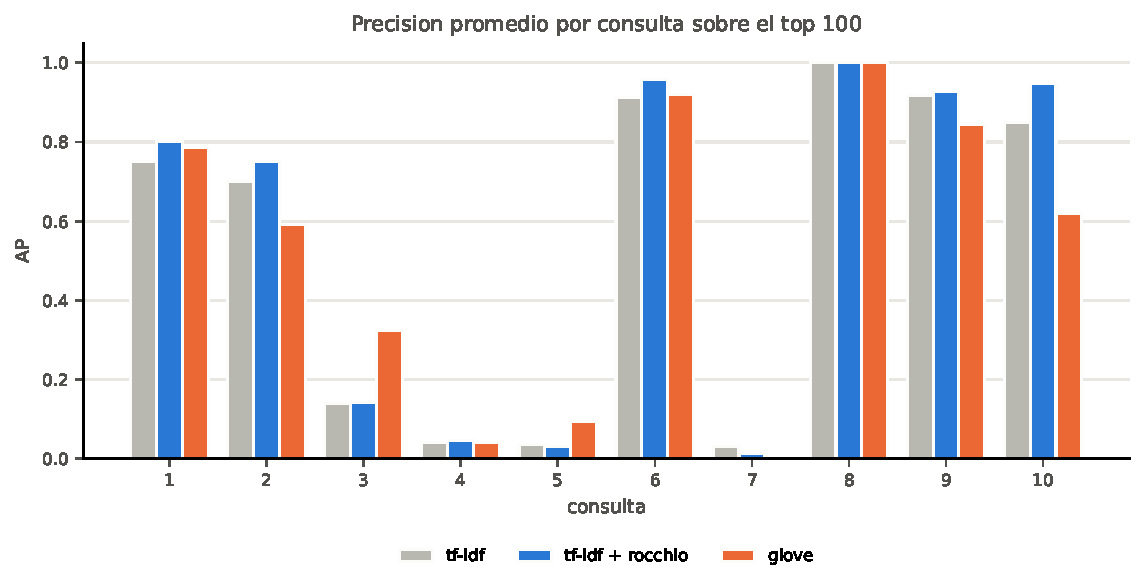
\includegraphics[width=0.85\linewidth]{glove_ap.pdf}
  \caption{AP por consulta de los tres sistemas.}
  \label{fig:ap}
\end{figure}

GloVe le gana a tf-idf en cinco consultas (1, 3, 4, 5 y 6), empata en
la 8 y pierde en cuatro (2, 7, 9 y 10). Las ganancias más grandes son
la 3, de $0.14$ a $0.32$, y la 5, de $0.04$ a $0.09$; las pérdidas más
grandes son la 10, de $0.85$ a $0.62$, y la 2, de $0.70$ a $0.59$. En
la 7 llega a cero

\section{Discusión}

\subsection*{Porque no se obtienen mejores resultados en todas?}

Creo que la diferencia depende de qué tipo de palabras trae cada
consulta

En la 3 y la 5 GloVe le gana a tf-idf, mi observacion con los resultados obtenidos es que estas
consultas describen un tema con palabras comunes, por ejemplo
\textit{persons involved in the viet nam coup}. Un documento relevante
puede hablar del golpe sin usar \texttt{persons} ni \texttt{involved},
y para tf-idf si la palabra no está, no cuenta. De hecho, en las dos
consultas hay un relevante que no comparte ningún término con la
consulta y que tf-idf nunca recupera. Con GloVe eso no pasa tanto,
porque \texttt{coup} queda cerca de palabras como \texttt{overthrow} o
\texttt{junta}, entonces un documento que usa esas palabras también se
acerca a la consulta. En la 5, por ejemplo, los primeros relevantes
suben de las posiciones 17 y 28 a la 6 y la 8.

En la 7 y la 10 pasa lo contrario, y en base a las observaciones la intuicion 
podria decir que es por los nombres propios. La 7 depende casi toda de \texttt{norodom sihanouk}, que
aparece en solo 4 documentos de la colección, así que en tf-idf tiene
un idf alto y pesa mucho. Pero al promediar, esas dos palabras valen lo
mismo que \texttt{further} o \texttt{nation}, y el nombre se pierde
entre las demás. Los dos relevantes terminan en las posiciones 101 y
172, fuera del top 100, y por eso el AP sale en cero. Con la 10 me
parece que pasa algo parecido con \texttt{malaysia}, que queda mezclada
con palabras como \texttt{growing} o \texttt{proposed}, y los dos
últimos relevantes bajan de las posiciones 8 y 9 a la 29 y la 46.

\section{Conclusiones}

Con el promedio de vectores GloVe el MAP es de $0.5221$, por debajo
de tf-idf ($0.5376$) y de tf-idf con Rocchio ($0.5618$). No es una
mejor representación para esta colección, pero tampoco es peor en
todo sino que es complementaria. Gana donde la consulta y los documentos usan
palabras distintas para el mismo tema, y pierde donde la consulta
depende de un nombre propio o de un término raro, que es justo donde
tf-idf es fuerte.

Se puede concluir que el problema no está en GloVe sino en el promedio,
que trata igual a \texttt{sihanouk} que a \texttt{further}.

\section*{Entregables}

\begin{center}
\begin{tabular}{ll}
    \toprule
    \texttt{out/actividad\_4/ap\_por\_consulta.csv}
      & AP por consulta de los tres sistemas \\
    \bottomrule
\end{tabular}
\end{center}

El archivo trae una fila por consulta, con las columnas
\texttt{query}, \texttt{tf-idf}, \texttt{tf-idf + rocchio} y
\texttt{glove}, o sea 10 filas.

El código está en \texttt{src/actividad.ipynb} y el entorno en
\texttt{../requirements.txt}. Los vectores de GloVe no se versionan
por su tamaño; las instrucciones para descargarlos están al inicio de
la actividad 4 en el notebook.

\section*{Referencias}

\begin{enumerate}[label={[\arabic*]}, itemsep=0.3em, leftmargin=*]
    \item \textbf{GloVe.} Jeffrey Pennington, Richard Socher y
          Christopher Manning, \emph{GloVe: Global Vectors for Word
          Representation}, EMNLP, 2014.\\
          \url{https://nlp.stanford.edu/projects/glove/}
    \item \textbf{Colección Time.} IR Group, University of Glasgow.
          Colecciones de prueba para recuperación de información.\\
          \url{http://ir.dcs.gla.ac.uk/resources/test_collections/}
\end{enumerate}

\end{document}

%############################ END OF REPORTE_4.TEX #############################
%###############################################################################
